\input ../preamble

\begin{document}

{\Huge
  \centerline{\bf TTIC 31230, Fundamentals of Deep Learning}
  \bigskip
  \centerline{David McAllester, Winter 2018}
  \vfill
  \centerline{\bf Stochastic Gradient Descent (SGD)}
  \vfill
  \centerline{The Classical Convergence Thoerem}
  \vfill
  \centerline{RMSProp, Momentum and Adam}
  \vfill
  \centerline{Scaling Learnng Rates with Batch Size}
  \vfill
  \centerline{SGD as MCMC and MCMC as SGD}
  \vfill
  \centerline{An Original SGD Algorithm}

\slide{Vanilla SGD}

$$\Phi \;\minuseq\; \eta \hat{g}$$

\vfill
\begin{eqnarray*}
  \hat{g} & = & E_{(x,y) \sim \mathrm{Batch}}\;\nabla_\Phi\;\mathrm{loss}(\Phi,x,y) \\
  \\
  \\
  g & = & E_{(x,y) \sim \mathrm{Train}}\;\nabla_\Phi\;\mathrm{loss}(\Phi,x,y) \\
\end{eqnarray*}

\vfill
For theoretical analysis we will focus on the case where the training data is very large --- essentially infinite.

\slide{Issues}

\vfill
\begin{itemize}
\item {\bf Gradient Estimation.} The accuracy of $\hat{g}$ as an estimate of $g$.

  \vfill
\item {\bf Gradient Drift (second order structure).} The fact that $g$ changes as the parameters change.
\end{itemize}

\slide{A One Dimensional Example}

Suppose that $y$ is a scalar, and consider

\vfill
$$\mathrm{loss}(\beta,x,y) = \frac{1}{2}(\beta - y)^2$$

\vfill
\begin{eqnarray*}
  g & = & E_{(x,y) \sim \mathrm{Train}}\; d\;\mathrm{loss}(\beta,x,y)/d \beta \;\;=\;\;\beta - E_{\mathrm{Train}}[y] \\
  \\
  \\
  \hat{g} & = & E_{(x,y) \sim \mathrm{Batch}} \; d\;\mathrm{loss}(\beta,x,y)/d \beta \;\;=\;\;\beta - E_{\mathrm{Batch}}[y]
\end{eqnarray*}

\slide{SGD as MCMC --- The SGD Stationary Distribution}

For small batches we have that each step of SGD makes a random move in parameter space.

\vfill
Even if we start at the training loss optimum, an SGD step will move away from the optimum.

\vfill
SGD defines an MCMC process with a stationary distribution.

\vfill
To converge to a local optimum the learning rate must be gradually reduced to zero.


\slide{The Classical Convergence Theorem}

$$\Phi \;\minuseq \; \eta^t \nabla_\Phi\;\mathrm{loss}(\Phi,x_t,y_t)$$

\vfill
For ``sufficiently smooth'' non-negative loss with

\vfill
$$\eta^t > 0\;\;\;\;\mbox{and}\;\;\;\;\lim_{t \rightarrow 0} \;\eta^t = 0\;\;\;\;\mbox{and}\;\;\;\;\sum_t \eta^t = \infty,$$

\vfill
we have that the training loss of $\Phi$ converges (in practice $\Phi$ converges to a local optimum of training loss).

\vfill
{\Large {\bf Rigor Police:} One can construct cases where $\Phi$ converges to a saddle point or even a limit cycle.}

\vfill
{\Large See ``Neuro-Dynamic Programming'' by Bertsekas and Tsitsiklis proposition 3.5.}

\slide{Physicist's Proof of the Convergence Theorem}

Since $\lim_{t \rightarrow 0} \;\eta^t = 0$ we will eventually get to arbitrarilly small learning rates.

\vfill
For sufficiently small learning rates any meaningful update of the parameters will be based on an arbitrarily large sample
of gradients at essentially the same parameter value.

\vfill
An arbitrarily large sample will become arbitrarily accurate as an estimate of the full gradient.

\vfill
But since $\sum_t \eta^t = \infty$, no matter how small the learning rate gets, we still can make arbitrarily large motions in parameter space.

\slide{Statistical Intuitions for Learning Rates}

For intuition consider the one dimensional case.

\vfill
At a fixed parameter setting we can sample gradients.

\vfill
Averaging together $N$ sample gradients produces a confidence interval on the true gradient.

$$g = \hat{g} \pm \frac{2\sigma}{\sqrt{N}}$$

To have the right direction of motion this interval should not contain zero.  This gives.

$$N \geq \frac{2\sigma^2}{\hat{g}^2}$$

\slide{Statistical Intuitions for Learning Rates}

$$N \geq \frac{2\sigma^2}{\hat{g}^2}$$

\vfill
To average $N$ gradients we need that $N$ gradient updates have a limited influence on the gradient.  

\vfill
This suggests
$$\eta^t \propto \frac{1}{N} \propto \frac{(g^t)^2}{(\sigma^t)^2}$$

\vfill
The constant of proportionality will depend on the rate of change of the gradient (the second derivative of loss).

\slide{Statistical Intuitions for Learning Rates}

$$\eta^t \propto \frac{(g^t)^2}{(\sigma^t)^2}$$

\vfill
This is written in terms of the true (average) gradient $g^t$ at time $t$ and the true standard deviation $\sigma^t$ at time $t$.

\vfill
This formulation is of conceptual interest but is not (yet) directly implementable (more later).

\vfill
As $g^t \rightarrow 0$ we expect $\sigma^t \rightarrow \sigma > 0$ and hence $\eta^t \rightarrow 0$.


\slide{Running Averages}

We can try to estimate $g^t$ and $\sigma^t$ with a running average.

\vfill
It is useful to review general running averages.

\vfill
Consider a time series $x_1$, $x_2$, $x_3$, $\ldots$.

\vfill
Suppose that we want to approximate a running average

$$\hat{\mu}_{t} \approx \frac{1}{N} \sum_{s=t-N+1}^t x_s$$

\vfill
This can be done efficiently with the update

\vfill
$$\hat{\mu}_{t+1} = \left(1-\frac{1}{N}\right)\hat{\mu}_t + \left(\frac{1}{N}\right)x_{t+1}$$

\slide{Running Averages}

More explicitly, for $\hat{\mu}_0 = 0$, the update

$$\hat{\mu}_{t+1} = \left(1-\frac{1}{N}\right)\hat{\mu}_t + \left(\frac{1}{N}\right)x_{t+1}$$

\vfill
gives

$$\hat{\mu}_t = \frac{1}{N} \sum_{1 \leq s \leq t} \left(1-\frac{1}{N}\right)^{-(t-s)} x_s$$

\vfill
where we have

$$\sum_{n\geq 0} \left(1-\frac{1}{N}\right)^{-n} = N$$


\slide{Back to Learning Rates}

In high dimension we can apply the statistical learning rate argument to each dimension (parameter) $\Phi[c]$ of the parameter vector $\Phi$ giving a separate learning rate for each dimension.

\vfill
$$\eta^t[c] \propto \frac{g^t[c]^2}{\sigma^t[c]^2}$$

\vfill
\begin{eqnarray*}
  \Phi^{t+1}[c] & = & \Phi^t[c] - \eta^t[c]\Phi^t[c]
\end{eqnarray*}


\slide{RMSProp}

RMS --- Root Mean Square --- was introduced by Hinton and proved effective in practice. We start by computing a running average of $\hat{g}[c]^2$.

$$s^{t+1}[c] = \beta s^t[c] + \left(1-\beta\right) \hat{g}[c]^2$$

\vfill
The PyTorch Default for $\beta$ is .99 which corresponds to a running average of 100 values of $\hat{g}[c]^2$.

\vfill
If $g^t[c] << \sigma^t[c]$ then $s^t[c] \approx \sigma^t[c]^2$.

\vfill
RMSProp:

$$\eta^t[c] \propto 1/\sqrt{s^t[c] + \epsilon}$$

\slide{RMSProp}

\vfill
RMSProp

\vfill
$$\eta^t[c] \propto 1/\sqrt{s^t[c] + \epsilon}$$

\vfill
bears some similarity to

\vfill
$$\eta^t[c] \propto g^t[c]^2/\sigma^t[c]^2$$

\vfill
but there is no attempt to estimate $g^t[c]$.

\slide{Momentum}

\centerline{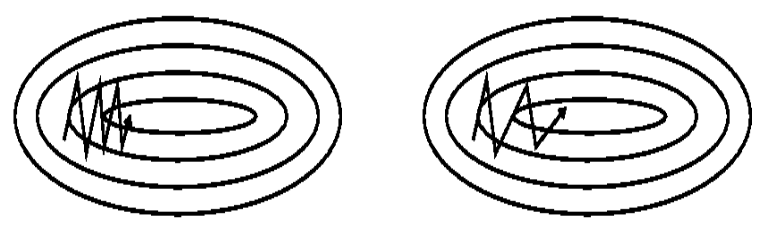
\includegraphics[width = 6in]{../images/momentum}}
\centerline{\Large Rudin's blog}

\vfill
The theory of momentum is generally given in terms of {\bf gradient drift} (the second order structure of total training loss).

\vfill
I will instead analyze momentum as a running average of $\hat{g}$.

\slide{Momentum, Nonstandard Parameterization}

\begin{eqnarray*}
  \tilde{g}^{t+1} & = & \mu \tilde{g}^t + (1-\mu)\hat{g}  \;\;\;\;\;\;\;\mu\in (0,1)\;\;\;\mbox{Typically}\;\mu \approx .9 \\
  \\
  \Phi^{t+1} & = & \Phi^t - \eta\tilde{g}^{t+1} \\
\end{eqnarray*}

\vfill
For $\mu = .9$ we have that $\tilde{g}^t$ approximates a running average of 10 values of $\hat{g}$.

\slide{Running Averages Revisited}

Consider any sequence $y_t$ derived from $x_t$ by

$$y_{t+1} = \left(1-\frac{1}{N}\right) y_t + f(x_t)\;\;\;\;\mbox{for any function $f$}$$

\vfill
We note that any such equation defines a running average of $Nf(x_t)$.

$$y_{t+1} = \left(1-\frac{1}{N}\right)y_t + \left(\frac{1}{N}\right)(N f(x_t))$$

\slide{Momentum, Standard Parameterization}

\begin{eqnarray*}
  v^{t+1} & = & \mu v^t + \eta * \hat{g}  \;\;\;\;\;\;\;\;\mu \in (0,1) \\
  \\
  \Phi^{t+1} & = & \Phi^t -  v^{t+1} \\
\end{eqnarray*}


\vfill
By the preceding slide $v^t$ is a running average of $(\eta/(1-\mu))\hat{g}$ and hence the above definition is equivalent to

\begin{eqnarray*}
  \tilde{g}^{t+1} & = & \mu \tilde{g}^t + (1-\mu) \hat{g}  \;\;\;\;\;\;\;\;\mu \in (0,1) \\
  \\
  \Phi^{t+1} & = & \Phi^t -  \left(\frac{\eta}{1-\mu}\right)\tilde{g}^{t+1} \\
\end{eqnarray*}

\slideplain{Momentum}

\begin{eqnarray*}
  \tilde{g}^{t+1} & = & \mu \tilde{g}^t + (1-\mu) \hat{g}  \;\;\;\;\;\;\;\;\mu \in (0,1),\;\mbox{typically .9} \\
  \\
  \Phi^{t+1} & = & \Phi^t -  \left(\frac{\eta}{1-\mu}\right)\tilde{g}^{t+1} \;\;\;\mbox{standard parameterization}\\
  \\
  \Phi^{t+1} & = & \Phi^t -  \eta'\tilde{g}^{t+1} \;\;\;\;\;\;\;\;\;\;\mbox{nonstandard parameterization}\\
\end{eqnarray*}

\vfill
The total contribution of a gradient value $\hat{g}^t$ is $\eta/(1-\mu)$ in the standard parameterization
and is $\eta'$ in the nonstandard parameterization (independent of $\mu$).
This suggests that the optimal value of $\eta'$ is independent of $\mu$ and that the $\mu$ does nothing.

\slideplain{Adam --- Adaptive Momentum}

\begin{eqnarray*}
  \tilde{g}^{t+1}[c] & = & \beta_1\tilde{g}^t[c] + (1-\beta_1) \hat{g}[c] \;\;\;  {\Large \mbox{PyTorch Default:}\;\beta_1 = .9} \\
  \\
  s^{t+1}[c] & = & \beta_2 s^t[c] + (1-\beta_2) \hat{g}[c]^2 \;\;\;{\Large \mbox{PyTorch Default:}\;\beta_2 = .999}\\
  \\
\Phi^{t+1}[c] & \minuseq & \frac{l_r}{\sqrt{(1-\beta_2^t)s^{t+1}[c]} + \epsilon}\;\; (1-\beta_1^t)\tilde{g}^{t+1}[c]
\end{eqnarray*}

\vfill
Given the argument that momentum does nothing, this should be
equivalent to RMSProp.  However, implementations of RMSProp and Adam differ in details such as default parameter values
and, perhaps most importantly, RMSProp lacks the ``initial bias correction terms'' $(1-\beta^t)$ (see the next slide).

\slideplain{Bias Correction in Adam}

Adam takes $\tilde{g}^0 = s^0 = 0$.

\vfill
For $\beta_2 = .999$ we have that $s^t$ is very small for $t << 1000$.

\vfill
To make $s^t[c]$ a better average of $g^t[c]^2$ we replace $s^t[c]$ by $(1-\beta_2^t)s^t[c]$.

\vfill
For $\beta_2 = .999$ we have $\beta_2^t \approx \exp(-t/1000)$ and for $t >> 1000$ we have $(1-\beta_2^t) \approx 1$.

\vfill
Similar comments apply to replacing $g^t[c]$ by $(1-\beta_1^t)g^t[c]$.

\slide{Learning Rate Scaling}

Recent work has show that by scaling the learning rate with the batch size very large batch size can lead to very fast (highly parallel)
training.

\vfill
{\bf Accurate, Large Minibatch SGD: Training ImageNet in 1 Hour}, Goyal et al., 2017.

\slide{Learning Rate Scaling}

Consider two consecutive updates for a batch size of 1 with learning rate $\eta_1$.

\begin{eqnarray*}
  \Phi^{t+1} & = & \Phi^t - \eta_1 \nabla_\Phi \mathrm{loss}(\Phi^t,x^t,y^t) \\
  \\
  \Phi^{t+2} & = & \Phi^{t+1} - \eta_1 \nabla_\Phi \mathrm{loss}(\Phi^{t+1},x^{t+1},y^{t+1}) \\\
  \\
  & \approx & \Phi^{t+1} - \eta_1 \nabla_\Phi \mathrm{loss}(\Phi^t,x^{t+1},y^{t+1}) \\
  \\
  & = & \Phi^t - \eta_1((\nabla_\Phi \mathrm{loss}(\Phi^t,x^t,y^t)) + (\nabla_\Phi \mathrm{loss}(\Phi^t,x^{t+1},y^{t+1})))
\end{eqnarray*}

\slide{Learning Rate Scaling}

Let $\eta_B$ be the learning rate for batch size $B$.

\vfill
\begin{eqnarray*}
  \Phi^{t+2} & \approx & \Phi^t - \eta_1((\nabla_\Phi \mathrm{loss}(\Phi^t,x^t,y^t)) + (\nabla_\Phi \mathrm{loss}(\Phi^t,x^{t+1},y^{t+1}))) \\
  \\
  & = & \Phi^t - 2\eta_1\;\hat{g}\;\;\;\mathrm{for}\;\;B=2
\end{eqnarray*}

\vfill
Hence two updates with $B=1$ at learning rate $\eta_1$ is the same as one update at $B=2$ and learning rate $2\eta_1$.

\vfill
$$\eta_2 = 2\eta_1,\;\;\;\;\;\;{\color{red} \eta_B = B\eta_1}$$
\slide{SGD as MCMC and MCMC as SGD}

\vfill
\begin{itemize}
\item {\bf Gradient Estimation.} The accuracy of $\hat{g}$ as an estimate of $g$.

  \vfill
\item {\bf Gradient Drift (second order structure).} The fact that $g$ changes as the parameters change.

  \vfill
\item {\bf Convergence.} To converge to a local optimum the learning rate must be gradually reduced toward zero.

  \vfill
  \item {\bf Exploration.} Since deep models are non-convex we need to search over the parameter space.  SGD can behave like MCMC.
\end{itemize}

\slide{Learning Rate as a Temperature Parameter}

\centerline{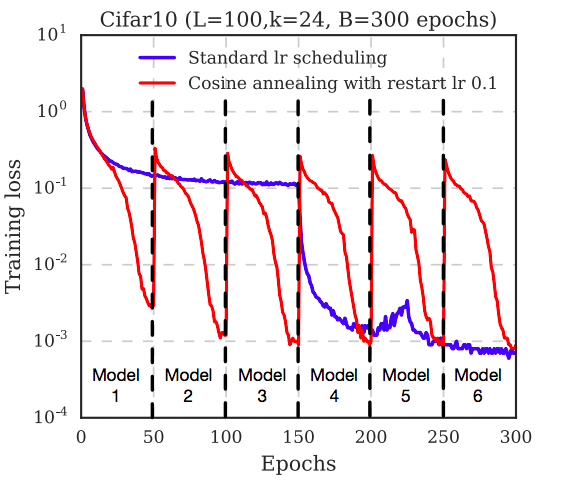
\includegraphics[height= 4in]{../images/AnnealingSGD}}
\centerline{\Large Gao Huang et. al., ICLR 2017}


\slide{Gradient Flow}

$$\mbox{Total Gradient Descent:} \;\;\Phi \;\minuseq\; \eta g$$

\vfill
Note this is $g$ and not $\hat{g}$. Gradient flow is defined by

\vfill
$$\frac{d \Phi}{d t} = - \eta g$$

\vfill
Given $\Phi(0)$ we can calculate $\Phi(t)$ by taking the limit as $N \rightarrow \infty$ of $Nt$ discrete-time total updates
$\Phi\; \minuseq \; \frac{\eta}{N} g$.


\vfill
The limit $N \rightarrow \infty$ of $Nt$ {\bf batch updates} $\Phi\; \minuseq \; \frac{\eta}{N} \hat{g}$ also gives $\Phi(t)$.

\slide{Gradient Flow Guarantees Progress}

\begin{eqnarray*}
  \frac{d \ell}{d t} & = & (\nabla_\Phi \;\ell(\Phi)) \cdot \frac{d \Phi}{dt} \\
  \\
  & = & - (\nabla_\Phi \;\ell(\Phi)) \cdot (\nabla_\Phi \;\ell(\Phi)) \\
  \\
  & = & - ||\nabla_\Phi \;\ell(\Phi)||^2 \\
  \\
  & \leq & 0
\end{eqnarray*}

\vfill
If $\ell(\Phi) \geq 0$ then $\ell(\Phi)$ must converge to a limiting value.

\vfill
This does not imply that $\Phi$ converges.

\slide{An Original Algorithm Derivation}

\vfill
We will derive a learning rate by maximizing a lower bound on the rate of reduction in training loss.

\vfill
We must consider

\vfill
\begin{itemize}
\item {\bf Gradient Estimation.} The accuracy of $\hat{g}$ as an estimate of $g$.

  \vfill
\item {\bf Gradient Drift (second order structure).} The fact that $g$ changes as the parameters change.
\end{itemize}

\slide{Analysis Plan}

We will calculate a batch size $B^*$ and learning rate $\eta^*$ by optimizing an improvement guarantee for a single batch update.

\vfill
We then use learning rate scaling to derive the learning rate  $\eta_B$ for a batch size $B << B^*$.

\slide{Deriving Learning Rates}

If we can calculate $B^*$ and $\eta^*$ for optimal loss reduction in a single batch
we can calculate $\eta_B$.

\vfill
$$\eta_B = B\;\eta_1$$

\vfill
$$\eta^* = B^* \eta_1$$

\vfill
$$\eta_1 = \frac{\eta^*}{B^*}$$

\vfill
$${\color{red} \eta_B = \frac{B}{B^*} \;\eta^*}$$

\slide{Calculating $B^*$ and $\eta^*$ in One Dimension}

We will first calculate values $B^*$ and $\eta^*$ by optimizing the loss reduction over a single batch update in one dimension.

\vfill
\begin{eqnarray*}
  g & = & \hat{g} \pm \frac{2\hat{\sigma}}{\sqrt{B}} \\
  \\
  \\
  \\
  \hat{\sigma} & = & \sqrt{E_{(x,y) \sim \mathrm{Batch}} \left(\frac{d\;\mathrm{loss}(\beta,x,y)}{d \beta} - \hat{g}\right)^2}
\end{eqnarray*}

\slide{The Second Derivative of $\mathrm{loss}(\beta)$}

\begin{eqnarray*}
  \mathrm{loss}(\beta) & = & E_{(x,y) \sim \mathrm{Train}}\;\mathrm{loss}(\beta,x,y) \\
  \\
  d^2 \mathrm{loss}(\beta)/d \beta^2 & \leq & L \;\;\;\mbox{\Large (Assumption)} \\
  \\
  \mathrm{loss}(\beta - \Delta\beta) & \leq & \mathrm{loss}(\beta) - g\Delta \beta + \frac{1}{2}L\Delta \beta^2 \\
  \\
  \\
  \mathrm{loss}(\beta - \eta\hat{g}) & \leq & \mathrm{loss}(\beta) - g(\eta\hat{g}) + \frac{1}{2}L(\eta\hat{g})^2
\end{eqnarray*}

\slide{A Progress Guarantee}

\begin{eqnarray*}
  \mathrm{loss}(\beta - \eta\hat{g}) & \leq & \mathrm{loss}(\beta) - g(\eta\hat{g}) + \frac{1}{2}L(\eta\hat{g})^2 \\
  \\
  \\
  & = &  \mathrm{loss}(\beta) - \eta (\hat{g} - (\hat{g} -g)) \hat{g} + \frac{1}{2}L\eta^2 \hat{g}^2 \\
  \\
  \\
  & \leq &  \mathrm{loss}(\beta) - \eta \left(\hat{g} - \frac{2\hat{\sigma}}{\sqrt{B}}\right)\hat{g} + \frac{1}{2}L \eta^2 \hat{g}^2
\end{eqnarray*}

\slideplain{Optimizing $B$ and $\eta$}

$$\mathrm{loss}(\beta - \eta\hat{g}) \leq \mathrm{loss}(\beta) - \eta \left(\hat{g} - \frac{2\hat{\sigma}}{\sqrt{B}} \right)\hat{g}  + \frac{1}{2}L \eta^2 \hat{g}^2$$

\vfill
We optimize progress per gradient calculation by optimizing the right hand side divided by $B$.  The derivation at the end of the slides gives

\vfill
$$B^*  =  \frac{16\hat{\sigma}^2}{\hat{g}^2},\;\;\;\;\eta^*  =  \frac{1}{2L}$$

\vfill
$${\color{red} \eta_B} = \frac{B}{B^*} \eta^* = {\color{red} \frac{B \hat{g}^2}{32\hat{\sigma}^2L}}$$

\vfill
Recall this is all just in one dimension.

\slide{Estimating $\hat{g}_{B^*}$ and $\hat{\sigma}_{B^*}$}

$${\color{red} \eta_B = \frac{B \hat{g}^2}{32\hat{\sigma}^2L}}$$

\vfill
We are left with the problem that $\hat{g}$ and $\hat{\sigma}$ are defined in terms of batch size $B^* >> B$.

\vfill
We can estimate $\hat{g}_{B^*}$ and $\hat{\sigma}_{B^*}$ using a running average with a time constant corresponding to $B^*$.

\slide{Estimating $\hat{g}_{B^*}$}

\begin{eqnarray*}
  \hat{g}_{B^*} & = & \frac{1}{B^*} \sum_{(x,y) \sim \mathrm{Batch}(B^*)}\; \frac{d\;\mathrm{Loss}(\beta,x,y)}{d\beta} \\
  \\
  \\
  & = & \frac{1}{N} \sum_{s=t-N+1}^t \hat{g}^s\;\;\;\;\;\mbox{with}\;N= \frac{B^*}{B} \;\mbox{for batch size}\;B \\
  \\
  \\
  \tilde{g}^{t+1} & = & \left(1-\frac{B}{B^*}\right)\tilde{g}^t + \frac{B}{B^*} \hat{g}^{t+1}
\end{eqnarray*}

\vfill
We are still working in just one dimension.

\slide{A Complete Calculation of $\eta$ (in One Dimension)}
\begin{eqnarray*}
  \tilde{g}^{t+1} & = & \left(1-\frac{B}{B^*(t)}\right)\tilde{g}^t + \frac{B}{B^*(t)} \hat{g}^{t+1} \\
  \\
  \tilde{s}^{t+1} & = & \left(1-\frac{B}{B^*(t)}\right)\tilde{s}^t + \frac{B}{B^*(t)} (\hat{g}^{t+1})^2 \\
  \\
  \tilde{\sigma}^t & = & \sqrt{\tilde{s}^t - (\tilde{g}^t)^2} \\
  \\
  B^*(t) &= & \left\{\begin{array}{ll} K & \mbox{for}\;\; t \leq K \\
  16(\tilde{\sigma}^t)^2/((\tilde{g}^t)^2 + \epsilon) & \mbox{otherwise} \end{array}\right.
\end{eqnarray*}

\slide{A Complete Calculation of $\eta$ (in One Dimension)}

$$\eta^t = \left\{\begin{array}{ll} 0 & \mbox{for}\;\;t \leq K \\ \frac{(\tilde{g}^t)^2}{32(\tilde{\sigma}^t)^2L} & \mbox{otherwise}
\end{array}\right.$$

\vfill
As $t \rightarrow \infty$ we expect $\tilde{g}^t \rightarrow 0$ and $\tilde{\sigma}^t \rightarrow \sigma > 0$ which implies
$\eta^t \rightarrow 0$.

\slide{The High Dimensional Case}

So far we have been considering just one dimension.

\vfill
We now propose treating each dimension $\Phi[c]$ of a high dimensional parameter vector $\Phi$ independently using the one dimensional analysis.

\vfill
We can calculate $B^*[c]$ and $\eta^*[c]$ {\bf for each individual parameter} $\Phi[c]$.

\vfill
Of course the actual batch size $B$ will be the same for all parameters.

\slide{A Complete Algorithm}
\begin{eqnarray*}
  \tilde{g}^{t+1}[c] & = & \left(1-\frac{B}{B^*(t)[c]}\right)\tilde{g}^t[c] + \frac{B}{B^*(t)[c]} \hat{g}^{t+1}[c] \\
  \\
  \tilde{s}^{t+1}[c] & = & \left(1-\frac{B}{B^*(t)[c]}\right)\tilde{s}^t[c] + \frac{B}{B^*(t)[c]} \hat{g}^{t+1}[c]^2 \\
  \\
  \tilde{\sigma}^t[c] & = & \sqrt{\tilde{s}^t[c] - \tilde{g}^t[c]^2} \\
  \\
  B^*(t)[c] &= & \left\{\begin{array}{ll} K & \mbox{for}\;\; t \leq K \\
  \lambda_B\tilde{\sigma}^t[c]^2/(\tilde{g}^t[c]^2 + \epsilon) & \mbox{otherwise} \end{array}\right.
\end{eqnarray*}

\slide{A Complete Algorithm}

$$\eta^t[c] = \left\{\begin{array}{ll} 0 & \mbox{for}\;\;t \leq K \\
        \frac{\lambda_\eta\tilde{g}^t[c]^2}{\tilde{\sigma}^t[c]^2} & \mbox{otherwise}
\end{array}\right.$$

\vfill
$$\Phi^{t+1}[c] = \Phi^t[c] - \eta^t[c] \hat{g}^t[c]$$

\vfill
Here we have meta-parameters $K$, $\lambda_B$, $\epsilon$ and $\lambda_\eta$.

\slideplain{Appendix: Optimizing $B$ and $\eta$}

$$\mathrm{loss}(\beta - \eta\hat{g}) \leq \mathrm{loss}(\beta) - \eta \hat{g}\left(\hat{g} - \frac{2\hat{\sigma}}{\sqrt{B}} \right)  + \frac{1}{2}L \eta^2 \hat{g}^2$$

Optimizing $\eta$ we get

\begin{eqnarray*}
 \hat{g}\left(\hat{g} - \frac{2\hat{\sigma}}{\sqrt{B}} \right) & = & L \eta \hat{g}^2
\end{eqnarray*}


\begin{eqnarray*}
\eta^*(B) & = & \frac{1}{L}\left(1 - \frac{2\hat{\sigma}}{\hat{g}\sqrt{B}}\right)
\end{eqnarray*}

\vfill
Inserting this into the guarantee gives
$$\mathrm{loss}(\Phi - \eta \hat{g}) \leq \mathrm{loss}(\Phi) - \frac{L}{2}\eta^*(B)^2\hat{g}^2$$

\slide{Optimizing $B$}

Optimizing progress per sample, or maximizing $\eta^*(B)^2/B$, we get

\begin{eqnarray*}
\frac{\eta^*(B)^2}{B} & = & \frac{1}{L^2}\left(\frac{1}{\sqrt{B}} - \frac{2\hat{\sigma}}{\hat{g}B}\right)^2 \\
\\
0 & = &  - \frac{1}{2} B^{-\frac{3}{2}} + \frac{2\hat{\sigma}}{\hat{g}} B^{-2} \nonumber \\
\\
B^* & = & \frac{16\hat{\sigma}^2}{\hat{g}^2} \\
\\
\eta^*(B^*) = \eta^*  & = & \frac{1}{2L}
\end{eqnarray*}

\ignore{
\slide{Appendix II: A Formal Bound for the Vector Case}

We will prove that minibatch SGD for a {\bf sufficiently large batch size} (for gradient estimation) and a {\bf sufficient small learning rate} (to avoid gradient drift)
is guaranteed (with high probability) to reduce the loss.

\vfill
This guarantee has two main requirements.

\vfill
\begin{itemize}
\item A smoothness condition to limit gradient drift.

  \vfill
\item A bound on the gradient norm allowing high confidence gradient estimation.
\end{itemize}
  

\slide{Smoothness: The Hessian}

We can make a second order approximation to the loss.

\begin{eqnarray*}
  \ell(\Phi + \Delta \Phi) & \approx & \ell(\Phi) + g^\top \Delta \Phi + \frac{1}{2} \Delta \Phi^\top H \Delta \Phi \\
  \\
  g & = & \nabla_\Phi\;\ell(\Phi) \\
  \\
  H & = & \nabla_\Phi \nabla_\Phi\; \ell(\Phi)
\end{eqnarray*}


\slide{The Smoothness Condition}

We will assume

$$||H\Delta \Phi|| \leq L||\Delta \Phi||$$

We now have

\vfill
$$\Delta \Phi^\top H \Delta \Phi \leq L ||\Delta \Phi||^2$$

\vfill
Using the second order mean value theorem one can prove

\begin{eqnarray*}
  \ell(\Phi + \Delta \Phi)  & \leq &    \ell(\Phi) + g^\top \Delta \Phi + \frac{1}{2} L ||\Delta \Phi||^2
\end{eqnarray*}


\slide{A Concentration Inequality for Gradient Estimation}

Consider a vector mean estimator where the vectors $g_n$ are drawn IID.

$$g_n = \nabla_\Phi \ell_n(\Phi) \;\;\;\;\;\;\hat{g} = \frac{1}{k} \sum_{n=1}^k g_n \;\;\;\; \;\;\;\;\;\;\;\; g = \expectsub{n}{\nabla_\Phi\;\ell_n(\Phi)}$$

\vfill
{\bf If with probability 1 over the draw of $n$ we have $|(g_n)_i - g_i| \leq b$ for all $i$} then with probability of at least $1-\delta$ over the draw of the sample

\vfill

$$||\hat{g} - g|| \leq \frac{\eta}{\sqrt{k}} \;\;\;\;\;\;\;\;\;\;\;\;\;\; \eta = b\left(1 + \sqrt{2 \ln (1/ \delta) }\right)$$


\vfill
{\huge Norkin and Wets ``Law of Small Numbers as Concentration Inequalities ...'', 2012, theorem 3.1}

\begin{eqnarray*}
 \ell(\Phi + \Delta \Phi) & \leq &   \ell(\Phi) + g^\top \Delta \Phi + \frac{1}{2} L ||\Delta \Phi||^2 \\
  \\
\ell(\Phi - \eta\widehat{g}) & \leq & \ell(\Phi) - \eta g^\top \widehat{g} + \frac{1}{2}L \eta^2 ||\widehat{g}||^2\\
  \\
  & = &  \ell(\Phi) - \eta (\widehat{g} - (\widehat{g} -g))^\top \widehat{g} + \frac{1}{2}L\eta^2 ||\widehat{g}||^2 \\
  \\
  & = &  \ell(\Phi) - \eta ||\widehat{g}||^2 + \eta(\widehat{g} -g)^\top \widehat{g} + \frac{1}{2}L \eta^2 ||\widehat{g}||^2 \\
  \\
  & \leq &  \ell(\Phi) - \eta ||\widehat{g}||^2 + \eta\frac{\eta}{\sqrt{k}}||\widehat{g}|| + \frac{1}{2}L \eta^2 ||\widehat{g}||^2 \\
  \\
  & = & \ell(\Phi) - \eta ||\widehat{g}||\left(||\widehat{g}|| - \frac{\eta}{\sqrt{k}} \right)  + \frac{1}{2}L \eta^2 ||\widehat{g}||^2 \\
\end{eqnarray*}

\slideplain{Optimizing $\eta$}

Optimizing $\eta$ we get

\begin{eqnarray*}
 ||\widehat{g}||\left(||\widehat{g}|| - \frac{\eta}{\sqrt{k}} \right) & = & - L \eta ||\widehat{g}||^2
\end{eqnarray*}


\begin{eqnarray*}
\eta & = & \frac{1}{L}\left(1 - \frac{\eta}{||\widehat{g}||\sqrt{k}}\right)
\end{eqnarray*}

\vfill
Inserting this into the guarantee gives
$$\ell(\Phi - \eta \widehat{g}) \leq \ell(\Phi) - \frac{L}{2}\eta^2||\widehat{g}||^2$$

\slide{Optimizing $k$}

Optimizing progress per sample, or maximizing $\eta^2/k$, we get.

\begin{eqnarray*}
\frac{\eta^2}{k} & = & \frac{1}{L^2}\left(\frac{1}{\sqrt{k}} - \frac{2\hat{\sigma}}{||\widehat{g}||k}\right)^2 \\
\\
0 & = &  - \frac{1}{2} k^{-\frac{3}{2}} + \frac{2\hat{\sigma}}{||\widehat{g}||} k^{-2} \nonumber \\
\\
k & = & \left(\frac{22\hat{\sigma}}{||\widehat{g}||}\right)^2 \\
\\
\eta & = & \frac{1}{2L}
\end{eqnarray*}
}


\slide{END}

} \end{document}

